\section{Aufbau und Durchführung}
\label{sec:Durchführung}

Zur Messung der Zeemanaufspaktung der roten und der blauen Spektrallinie einer
Cd-Dampflampe steht der in Abbildung \ref{fig:aufbau} dargestellte Versuchsaufbau zur Verfügung.

\begin{figure}
  \centering
  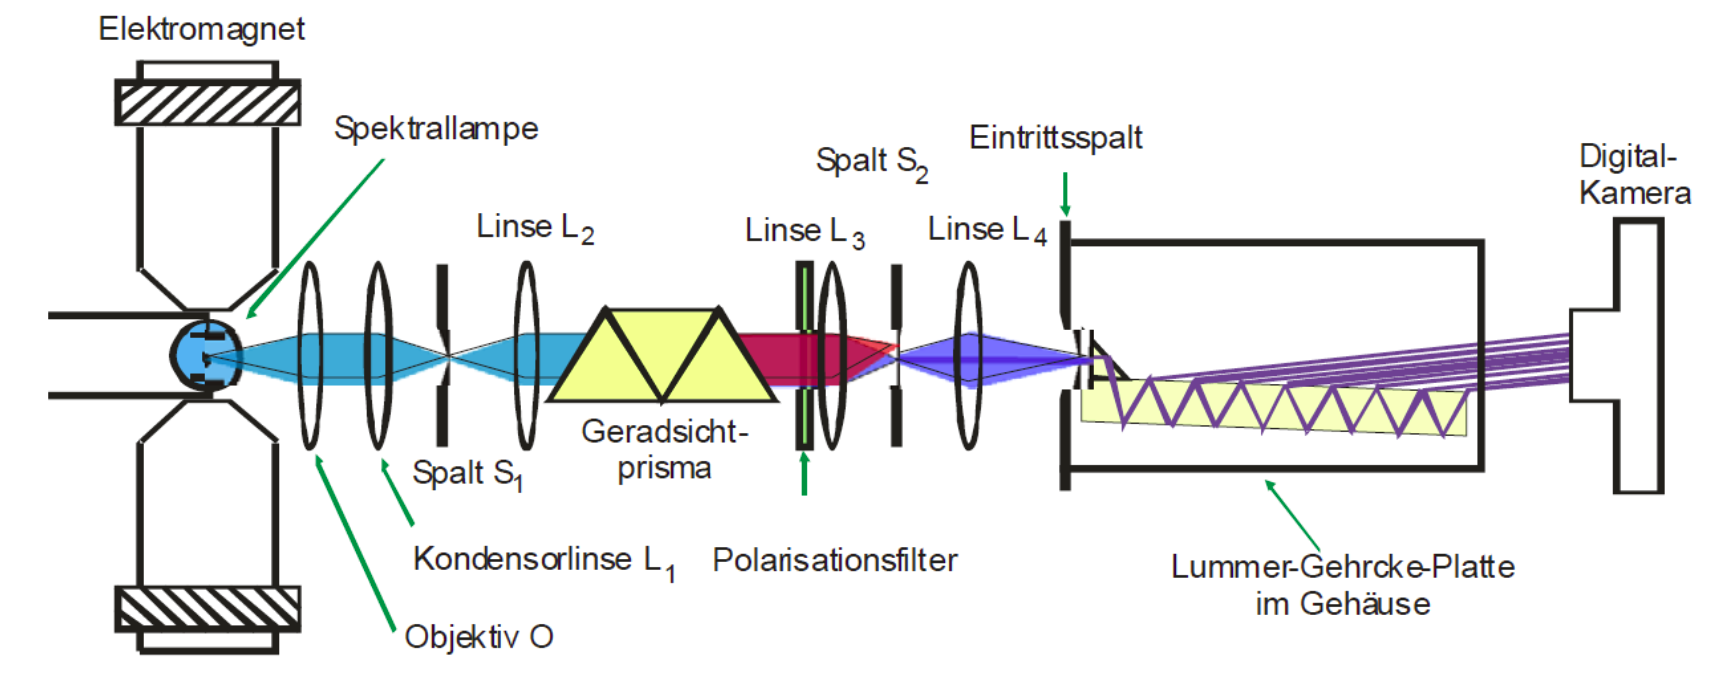
\includegraphics[width=\textwidth]{data/aufbau.png}
  \caption{Schematische Skizze des Versuchsaufbaus. \cite{Versuchsanleitung}}
  \label{fig:aufbau}
\end{figure}

Zu erkennen ist dort eine Cd-Lampe, die im Feld eines Elektromagneten steht. Transversal
zum Magnetfeld wird das emittierte Licht anschließend gebündelt und durch ein
Geradsichtprisma in seine Spektrallinien zerlegt. Anschließend kann die zu untersuchende
Wellenlänge mithilfe eines Interferenzfilters herausgefiltert werden. Das Licht dieser
Wellenlänge wird dann auf eine Lummer-Gehrcke-Platte gebündelt und das von dieser
erzeugt Interferenzmuster mit einer Kamera fotografiert.

Die Lummer-Gehrcke-Platte nutzt den Effekt der Interferenz an planparallelen Schichten aus.
Eine Skizze zur Funktionsweise einer Lummer-Gehrcke-Platte ist in Abbildung
\ref{fig:lummer} zu sehen.

\begin{figure}
  \centering
  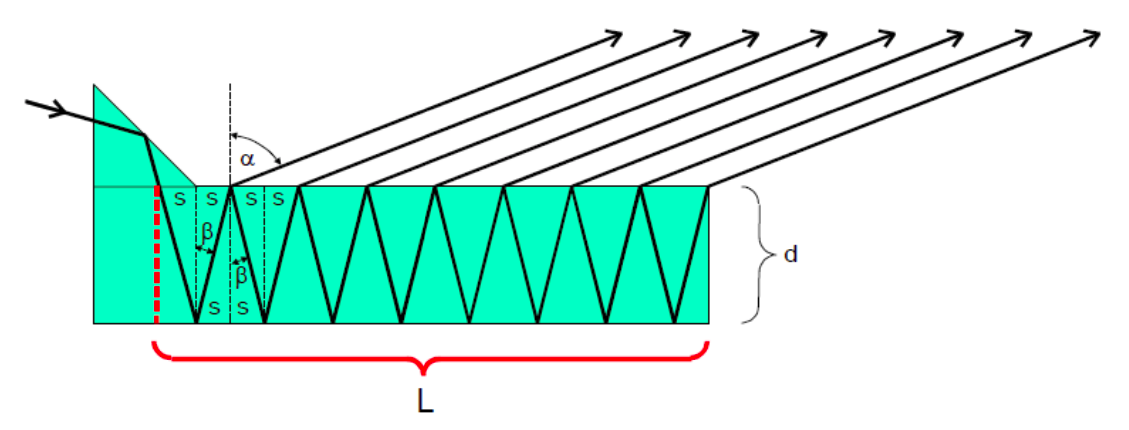
\includegraphics[width=\textwidth]{data/lummer.png}
  \caption{Skizze zur Funktionsweise einer Lummer-Gehrcke-Platte. \cite{Versuchsanleitung}}
  \label{fig:lummer}
\end{figure}

Mithilfe eines Prismas wird das Licht in eine dünne Platte reflektiert, in der
es anschließend hin und her refliektiert wird. Bei jeder Reflexion wird auch ein kleiner
Teil des Lichts transmittiert. Für konstruktive Interferenz gilt die Bedingung
\begin{equation}
  2n d \cos(\beta)=m \lambda,
\end{equation}
Wobei $n$ der Brechungsindex der Platte, $d$ die Dicke der Platte, $m$ eine natürliche
Zahl und $\lambda$ die Wellenlänge des eingestrahlten Lichts ist. Bei einer Bestrahlung einer
Lummer-Gehrcke-Platte mit monochromatischem Licht entstehen Interferenzstreifen, deren
Gangunterschied der eingestrahlten Wellenlänge entspricht. Bei einer Veränderung
des Magnetfeldes verändert sich die Wellenlänge der eingestrahlten Strahlung, sodass
sich auch die Interferenzstreifen verschieben.

Für große Austrittswinkel lässt sich der Spektralbereich $\Delta \lambda_D$ durch
den Ausdruck
\begin{equation}
   \Delta \lambda = \frac{\lambda^2}{2d} \sqrt{\frac{1}{n^2-1}}
\end{equation}
berechnen. Dabei ist $d$ die Dicke und $n$ der Brechungsindex der Lummer-Gehrcke-Platte.
Das Auflösungsvermögen einer Lummer-Gehrcke-Platte ist gegeben durch
\begin{equation}
  A = \frac{\lambda}{\increment \lambda} = \frac{L}{\lambda}(n^2-1) \,.
\end{equation}

Im Versuch wird zunächst die Apparatur möglichst genau justiert. Dafür werden
die Linsen so eingestellt, dass eine scharfe Abbildung auf die Lummer-Gehrcke-Platte
fällt. Durch Variation der Spaltbreite kann die Helligkeit gesteuert werden.
Anschließend wird ein Polarisationsfilter in den Strahlengang gebracht und es werden
mithilfe einer Kamera Bilder gemacht. Zunächst wird ein Bild von der roten Linie ohne
Magnetfeld und anschließend mit Magnetfeld für beide Polarisationsrichtungen gemacht.
Daraufhin wird für die blaue Spektrallinie analog verfahren.
